\chapter{Modelo Conceptual}
\label{chap:model}
%The project's conceptual model and the identification of all tasks implemented by the prototype
O modelo conceptual desenvolvido é visível na Figura \ref{fig:model}, foi construído tendo em consideração que o jogo seria um railshooter, isto é, um jogo em que se controla uma entidade num espaço bidimensional e cujo objectivos é sobreviver e alcançar o máximo de pontuação possível.

A medida que o jogo foi desenvolvido, algumas alterações foram feitas para que o modelo se aproximasse mais com que era desejado para passar a mensagem.
Sendo este o resultado final.

\begin{figure}[h]
\centering
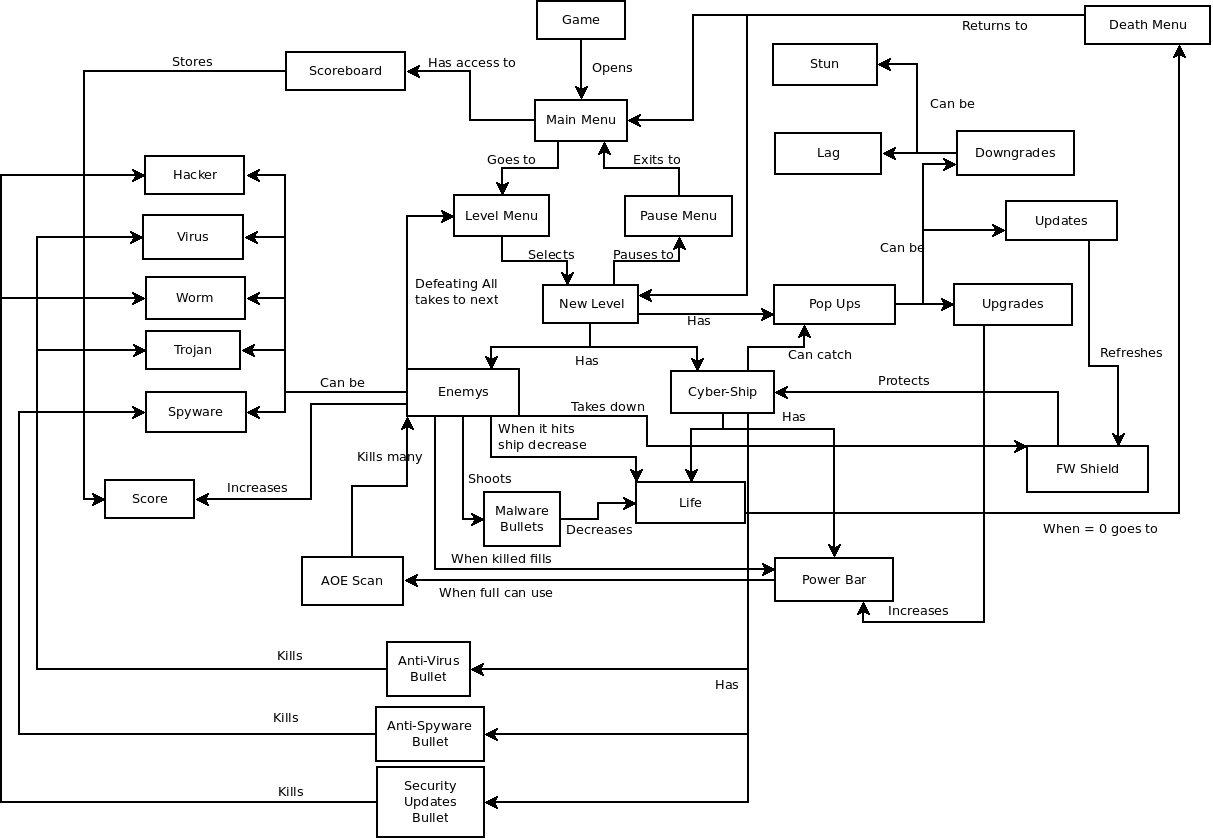
\includegraphics 
	[width = 0.75\textwidth] {ModeloConceptual}
\caption{\label{fig:model}} Modelo Conceptual
\end{figure}

Para o protótipo que foi criado decidimos implementar apenas partes das tarefas descritas acima, como é possível ver na Figura \ref{fig:demo}.

\begin{figure}[h]
\centering
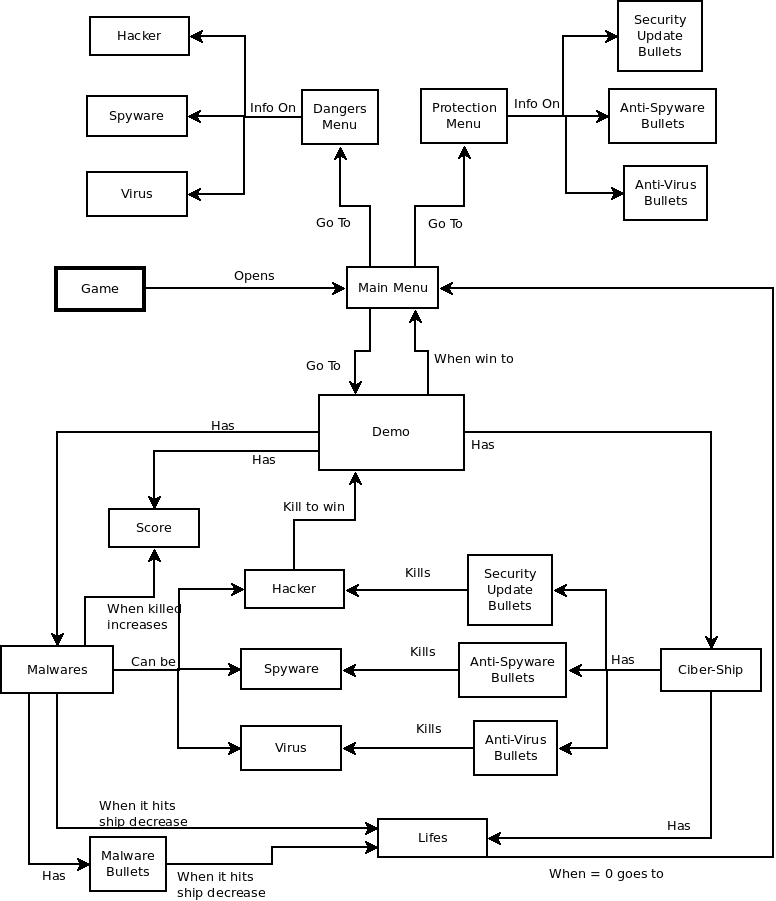
\includegraphics 
	[width = 0.75\textwidth] {DemoModeloConceptual}
\caption{\label{fig:demo}} Modelo Conceptual do Protótipo
\end{figure}

Começando pelas tarefas que não foram contempladas no protótipo final,
é possível ver que as secções referentes aos \textit{PopUps}, \textit{Upgrades} e \textit{Power Bar} não estão contempladas, já que não se considerou que contivesse importância suficiente para passar a mensagem.

Alguns \textit{Malwares} foram também excluídos, não devido à importância dos seus conteúdos mas sim para manter consistência na sequência da história do protótipo.
Sendo que, para que tal fosse possível, o Worm e o Trojan não foram incluídos.

O Scoreboard, onde a pontuação de todos os níveis seriam guardadas, também não foi implementa, pois implicaria guardar valores de forma permanente o que implicaria um esforço desnecessário, já que não se torna relevante quando se trata apenas de uma protótipo.

Todas as outras tarefas foram implementas no protótipo, seguindo este segundo modelo conceptual.